\documentclass[11pt,oneside]{book}
\usepackage[english]{babel} 
\usepackage{microtype}
\usepackage[utf8]{inputenc}
\usepackage{subfigure}
\usepackage{epsfig}
\usepackage{amsmath, amssymb}
\usepackage[linesnumbered,lined,commentsnumbered,italiano]{algorithm2e}
\usepackage{fancybox}
\usepackage{listings}
\usepackage{url}
\usepackage{graphicx}
\usepackage{todonotes}
\usepackage{moreverb}
\usepackage[labelfont=it,textfont={it}]{caption}
\usepackage[final,bookmarks,breaklinks,colorlinks,allcolors=black]{hyperref}
\usepackage{color}
\usepackage[block=ragged,backend=biber,natbib=true]{biblatex} % Use the bibtex backend with the authoryear citation style (which resembles APA)
\addbibresource{sections/04_bibliography.bib} % The filename of the bibliography
\usepackage[autostyle=true]{csquotes} % Required to generate language-dependent quotes in the bibliography


\definecolor{mygreen}{rgb}{0,0.6,0}
\definecolor{mygray}{rgb}{0.5,0.5,0.5}
\definecolor{mymauve}{rgb}{0.58,0,0.82}
\lstset{ %
	backgroundcolor=\color{white},   % choose the background color; you must add \usepackage{color} or \usepackage{xcolor}; should come as last argument
	basicstyle=\footnotesize,        % the size of the fonts that are used for the code
	breakatwhitespace=false,         % sets if automatic breaks should only happen at whitespace
	breaklines=true,                 % sets automatic line breaking
	captionpos=b,                    % sets the caption-position to bottom
	commentstyle=\color{mygreen},    % comment style
	deletekeywords={...},            % if you want to delete keywords from the given language
	escapeinside={\%*}{*)},          % if you want to add LaTeX within your code
	extendedchars=true,              % lets you use non-ASCII characters; for 8-bits encodings only, does not work with UTF-8
	frame=single,
	keepspaces=true,                 % keeps spaces in text, useful for keeping indentation of code (possibly needs columns=flexible)
	keywordstyle=\color{blue},       % keyword style
	morekeywords={*,...},            % if you want to add more keywords to the set
	numbers=left,                    % where to put the line-numbers; possible values are (none, left, right)
	numberstyle=\tiny\color{mygray}, % the style that is used for the line-numbers
	rulecolor=\color{black},         % if not set, the frame-color may be changed on line-breaks within not-black text (e.g. comments (green here))
	showspaces=false,                % show spaces everywhere adding particular underscores; it overrides 'showstringspaces'
	showstringspaces=false,          % underline spaces within strings only
	showtabs=false,                  % show tabs within strings adding particular underscores
	stringstyle=\color{mymauve},     % string literal style
	tabsize=2,	                   % sets default tabsize to 2 spaces
	title=\lstname                   % show the filename of files included with \lstinputlisting; also try caption instead of title
}


\definecolor{gray}{rgb}{0.4,0.4,0.4}
\definecolor{darkblue}{rgb}{0.0,0.0,0.6}
\definecolor{cyan}{rgb}{0.0,0.6,0.6}


\definecolor{javared}{rgb}{0.6,0,0} % for strings
\definecolor{javagreen}{rgb}{0.25,0.5,0.35} % comments
\definecolor{javapurple}{rgb}{0.5,0,0.35} % keywords
\definecolor{javadocblue}{rgb}{0.25,0.35,0.75} % javadoc


\lstdefinelanguage{FLY}
{
  morestring=[b]",
  morecomment=[l]{//},
  morecomment=[s]{/}{/},
  identifierstyle=\color{black},
  keywordstyle=\color{javapurple},
  morekeywords={func,var,while, if, then, else,for, in, println, fly ,on,thenall,as,then,require,native}% list your attributes here
}


\lstset{language=FLY,
basicstyle=\ttfamily\scriptsize,
keywordstyle=\color{javapurple}\bfseries,
stringstyle=\color{javared},
commentstyle=\color{javagreen},
morecomment=[s][\color{javadocblue}]{/*}{/},
numbers=left,
numberstyle=\tiny\color{black},
stepnumber=1,
numbersep=10pt,
tabsize=4,
showspaces=false,
showstringspaces=false}


\begin{document}
\begin{titlepage}
\begin{center}

\epsfig{file=figures/logo_standard.jpg,width=2.5truecm}\\[0.2truecm]
{\Large Universit\`a degli Studi di Salerno}\\[0.2truecm]
{\large Dipartimento di Informatica}\\
\hrulefill
\vfill
{\large Tesi di Laurea di I livello in }\\[0.2truecm]
{\Large Informatica}\\
\vfill\vfill
{\Huge Template tesi ISISLab}
\vfill\vfill


{\bf Relatore} \hfill {\bf Candidato}\ \ \\
Nome Cognome \hfill Nome Cognome\\
{\bf Correlatore} \hfill {\bf }\ \ \\
Dott. Nome Cognome \hfill \ \ \\

\vfill
\hrulefill 

Academic Year 2021-2022

\end{center}
\end{titlepage}

\pagenumbering{roman}
\chapter*{Abstract}
Lorem ipsum dolor sit amet, consectetur adipiscing elit, sed do eiusmod tempor incididunt ut labore et dolore magna aliqua. Ut enim ad minim veniam, quis nostrud exercitation ullamco laboris nisi ut aliquip ex ea commodo consequat. Duis aute irure dolor in reprehenderit in voluptate velit esse cillum dolore eu fugiat nulla pariatur. Excepteur sint occaecat cupidatat non proident, sunt in culpa qui officia deserunt mollit anim id est laborum.



\tableofcontents
\pagestyle{plain}

%%%%%%%%%%%%%%%%%%%%%%%%%%%%
\chapter{Introduction}
\setcounter{page}{1} 	% devono seguire solo il primo capitolo
\pagenumbering{arabic}	% devono seguire solo il primo capitolo

A computer hardware and software combination created for a particular purpose is an Embedded System (\es). In many cases, \ess operate as part of a bigger system (\eg  agricultural and processing sector equipment, automobiles, medical equipment, airplanes, and so on) and within tight resource constrains (\eg small battery capacity, limited memory and CPU speed, and so on).
The global \ess market is expected to witness notable growth. A recent report evaluated the global \ess market 89.1 billion dollars in 2021, and this market is projected to reach 163.2 billion dollars by 2031; with a compound annual growth rate of 6.5\%~ \cite{ESSTR2022}. This growth is mostly related to an increase in the demand for advanced driver-assistance system (in electric and hybrid vehicles) and in the number of \ess-related research and development projects.  
To date, there has yet to be shown which approach is to be preferred when developing \ess. For example, Greening \cite{TDDEC} in his book asserted that embedded developers can benefit from the application of
Test-Driven Development (\tdd), an incremental approach to software development in which a developer repeats a short development cycle made up of three phases: \textit{red}, \textit{green}, and \textit{blue/refactor} \cite{TDDByExample}. During the red phase, the developer writes a unit test for a small chunk of a functionality not yet implemented and watches the test fail. In the green phase, the developer implements the chunk of functionalities as quickly as possible and watches all the unit tests pass. During the refactoring phase, the developer changes the internal structure of the code while paying attention to keep the functionality intact—accordingly, all unit tests should pass. TDD has been conceived to develop “regular” software, and it is claimed to improve software quality as well as developers' productivity \cite{DBLP:reference/se/ErdogmusMJ10}. \ess have all the same challenges of non-embedded systems (\noess), such as poor quality, but add challenges of their own [6]. 
For example, one of the most cited differences between embedded and \noess is that embedded code depends on the hardware. While in principle, there is no difference between a dependency on a hardware device and one on a \noess \cite{TDDEC}, dealing with hardware introduces a whole new set of variables to consider during development. Furthermore, the limited resources on which an \es usually operates may make it extremely difficult to properly test the system in its entirety. 
Over the years, a huge amount of empirical investigations has been conducted to study the claimed effects of TDD on the development of \noess (\eg, \cite{DBLP:journals/software/KaracT18}). So far no investigations have been conducted to assess possible benefits concerned the application of TDD on the development of \ess although some authors, like Greening \cite{TDDEC}, believes that embedded developers can benefit from the application of TDD in the development of \ess.

In this work of thesis, we investigate the following primary research question (RQ):

\begin{framed}
\noindent \textbf{RQ.} To what extent does the use of \tdd impact the external quality, productivity, and number of test cases of the developed \es?	
\end{framed}

To answer this RQ, we present the results of an exploratory empirical assessment constituted of two experiment, a controlled experiment that acts as the baseline for the study, and its replication to study the application of \tdd on the implementation of \ess. The participants were final year Master's degree students in Computer Science enrolled to an \es course at the University of Salerno, in Italy. The goal of these experiments is to increase the body of knowledge on the benefit (if any) related to the application of \tdd in the context of the development of \ess. To that end, we compare \tdd with respect to a more traditional, test-last, development practice, where test cases are written after the production code. From here onwards, we refer to this traditional way of coding as \notdd. Whichever the used approach (\tdd and \notdd), the participants in the implementation of an \es where asked to use a mock to model and confirm the interactions between a device driver and the hardware. The mocked implementation would intercept commands to and from the device simulating a given usage scenario. In the replication experiment, the participants had to implement an additional \es with the end goal of replacing the mocks with real hardware components (a number of sensors and actuators) before deploying the \es on the actual hardware platform they had mocked up to that point. The logic of the \es was deployed on a Raspberry Pi model 4 board, and the developed test cases were executed in the real environment. Variations in the replicated experiments (task and the experimental procedure) were introduced to validate the results of the baseline experiment and to generalize these results to a more real setting. The results obtained by an aggregated analysis of the data from both the experiments suggest that there are no significant differences between \tdd and \notdd on: productivity, number of written tests, a..., respectively. On the other hand, we observed a significant difference on: ... When analyzing experiments individually, we observed that ...

As for the following thesis structure, it is made up of five chapters:
The first two act as the foundational knowledge concepts that provide a general overview on the main topics concerning the \tdd methodology and \es technologies: chapter one contains an overview on the software testing process, analyzing the main approaches, with a focus on \tdd. Chapter two will provide information on the general \ess concepts, enabling technologies and implementation challenges, before discussing the techniques for testing such systems.
In chapter three, we conduct a review of the literature by examining the most relevant previous empirical studies on the application of \tdd and the current testing methodologies for \es.
Chapter four will contain the detail explanation of our approach for the definition of the two experimental studies, the analysis of the results, and our answers to the research questions.
Finally, chapter five will provide the conclusions to the thesis, along with a discussion on the possible ramification the research could manifest when moving forward in the analysis of \tdd for \es development.
 
%%%%%%%%%%%%%%%%%%%%%%%%%%%%
\chapter{Literature}
When formulating the test case search problem as a many-objective optimisation problem, the goal is to minimize all the individual distances from all the test targets in the class under test.

One of the most popular multi-objective algorithms for this problem is the Non-dominated Sorting Genetic Algorithm II (NSGA-II). This algorithm is based on three principles:

\begin{itemize}
    \item It uses elitism when evolving the population: the most fit individuals are carried over along the offsprings.
    \item It uses an explicit diversity-preserving mechanism, the Crowding distance.
    \item It emphasizes the non-dominated solutions, as its name suggests.
\end{itemize}

First of all, in the context of test cases, domination can be expressed by the following relation:
\begin{figure}[h]
    \centering
    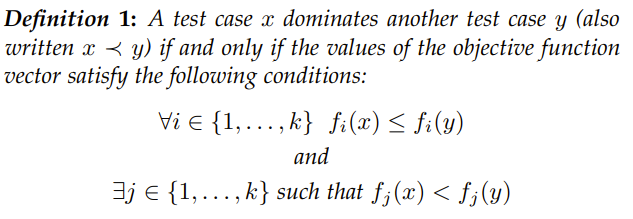
\includegraphics[scale=0.4]{./figures/test_Case_domination.PNG}
    \caption{Test case domination}
    \label{fig:test case domination}
\end{figure}


The NSGA-II algorithm works as follows:
\begin{itemize}
    \item Starting from an initial population of individuals Pt, generate an offspring population Qt of equal size and merge the two together, obtaining the population Rt.
    \item Perform non-dominated sorting of the individuals in Rt based on target indicatiors and classify them by fronts, i.e. the are sorted according to an ascending level of non-domination.  This ensures that the top Pareto-optimal individuals will survive to the next generation.
    \item If one of the fronts in the sorted sequence doesn't fit in terms of population size, crowding distance sorting is performed.
    \item Create the new population based on crowded tournament selection, then perform crossover and mutation. 
\end{itemize}


Figure 2.2 summarizes the main loop of the algorithm:
\begin{figure}[h]
    \centering
    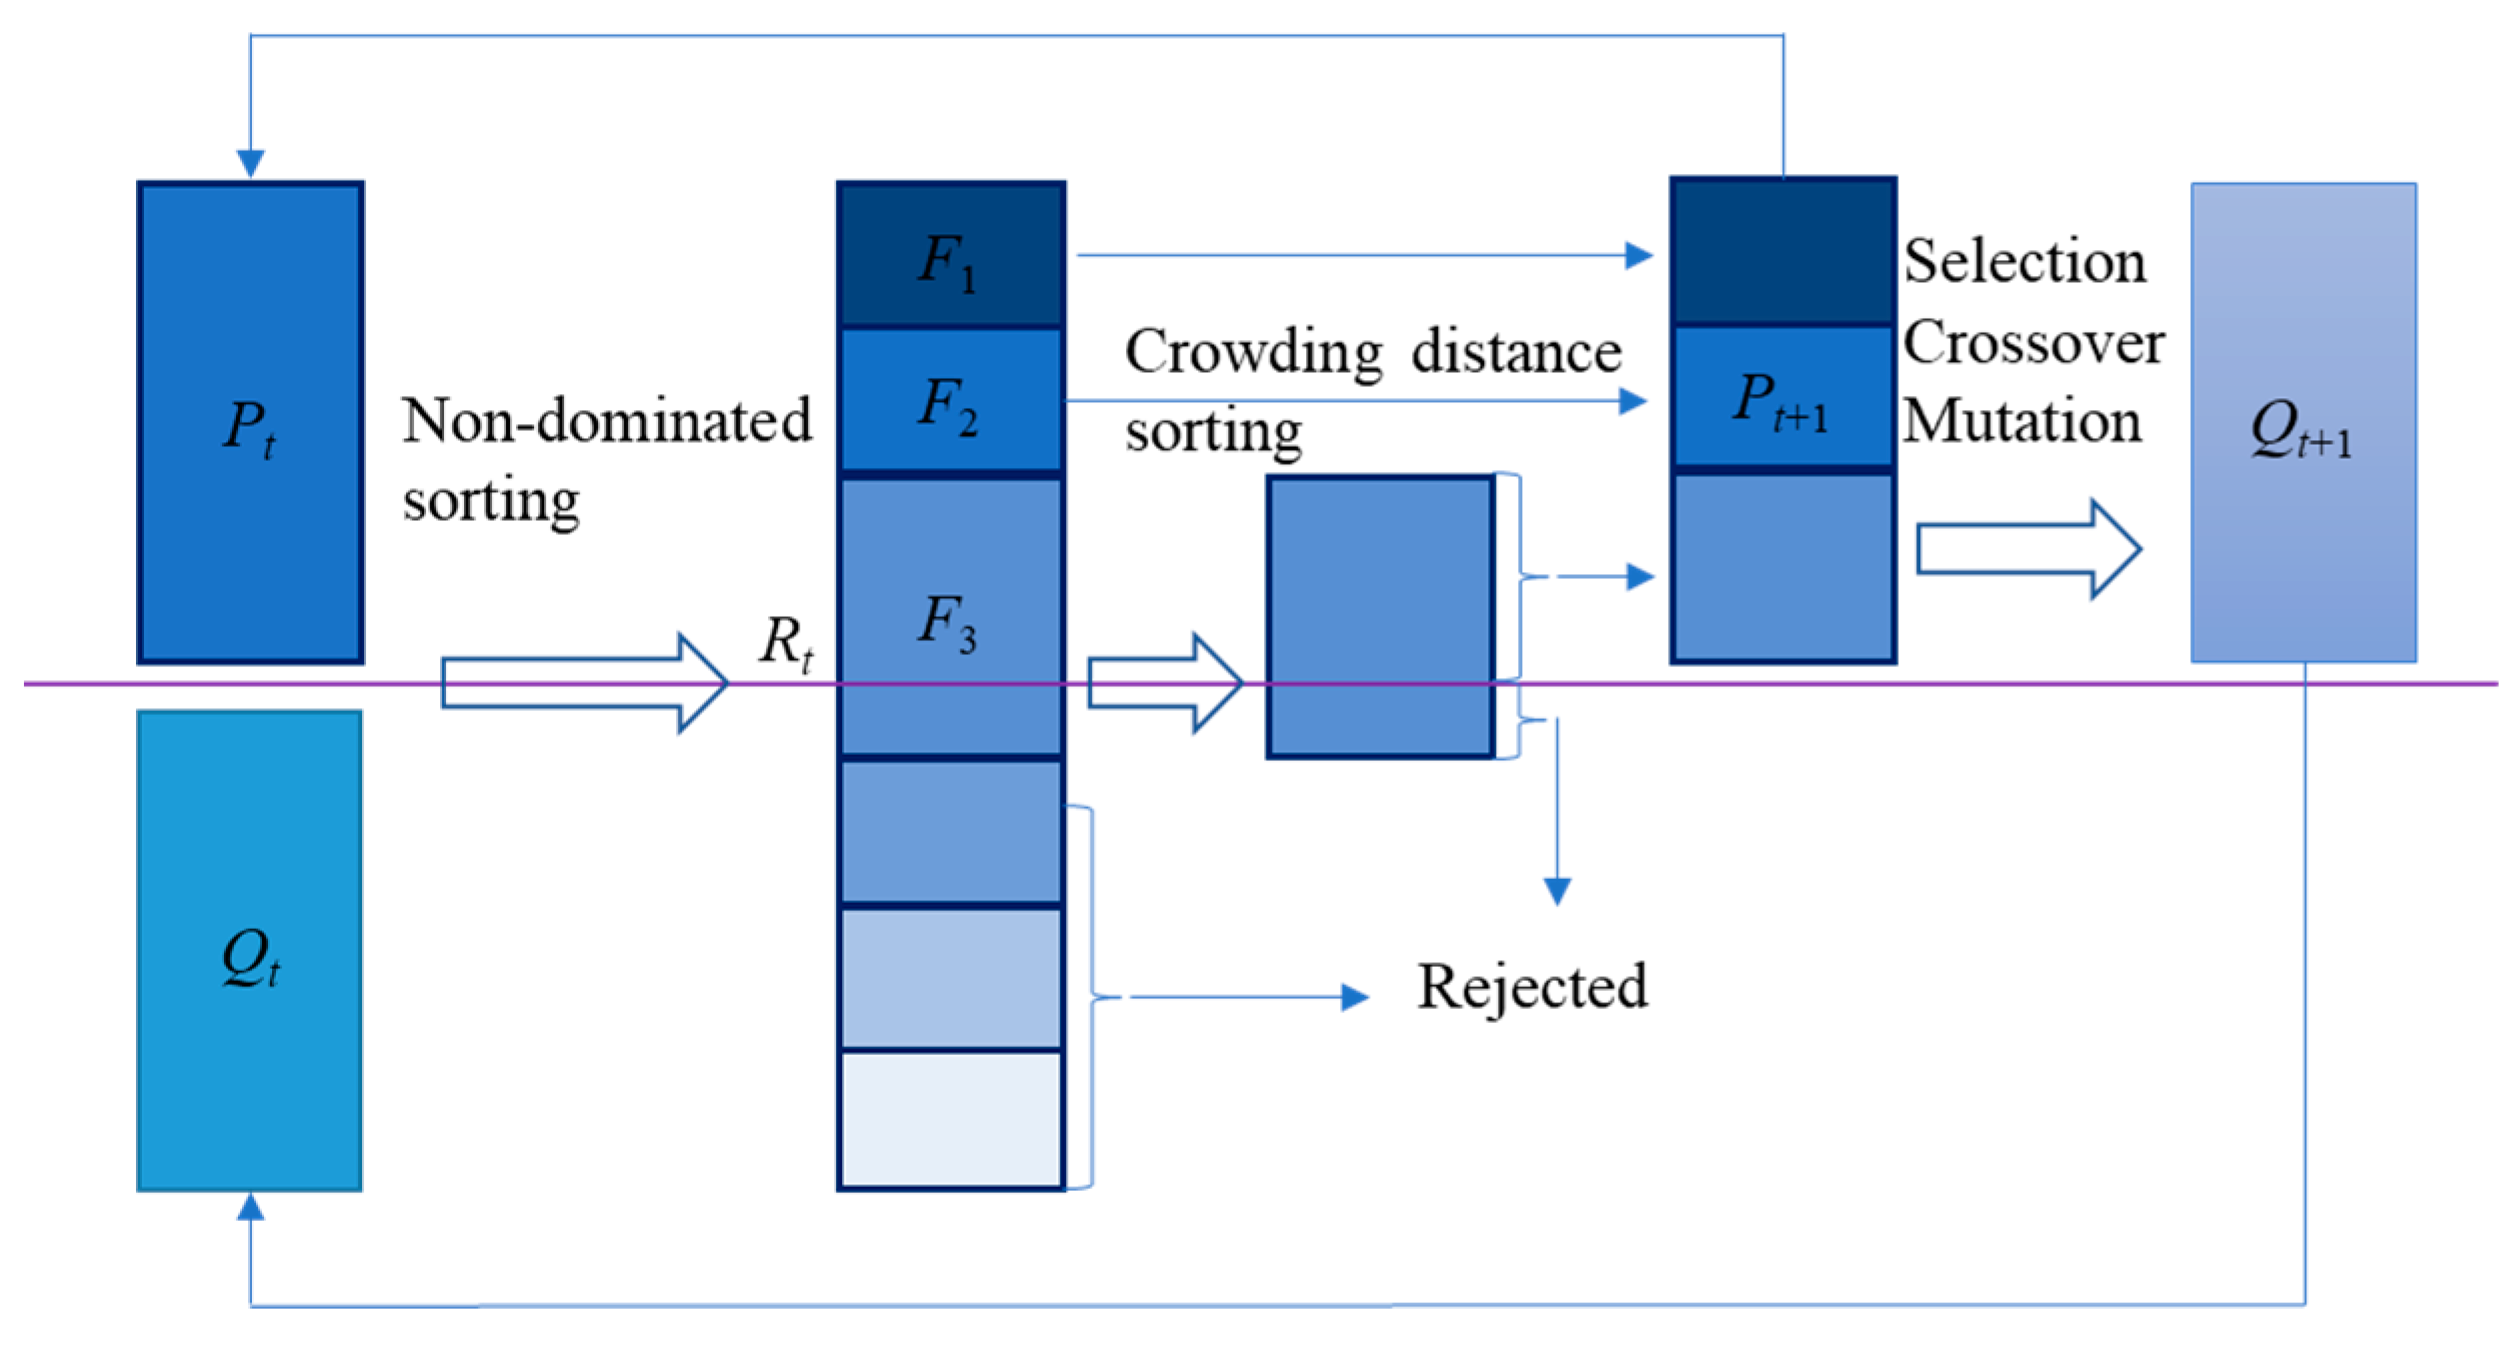
\includegraphics[scale=0.1]{./figures/nsga-ii.png}
    \caption{NSGA-II algorithm main loop}
    \label{fig:NSGA-II algorithm main loop}
\end{figure}


In the context of software enginnering, NSGA-II has been applied to problems such as software refactoring and test case prioritization,
with two or three objectives. If the number of objectives begins to grow, however, the performance of the algorithm doesn't scale up well \cite{article3}.
To overcome these limitation 


DynaMOSA, Dynamic Many-Objective Sorting Algorithm \cite{article1} is an approach that focuses on ..., and has been developed as an evolution of MOSA. This latter solution implements a many-objective GA to tackle test case generation and has three main features: 
\begin{itemize}
    \item instead of ranking candidates for selection based on their Pareto optimality, it uses a preference criterion. This criterion selects the test case with the lowest objective score for each uncovered target; these selected individuals are given a higher chance of survival, while other test cases are ranked with the traditional NSGA-II approach.
    \item The search is focused only on the uncovered coverage targets.
    \item All tests that satisfy one or more of the uncovered targets will be archived and used as the final test suite once the search ends.
\end{itemize}

In many-objective optimisation problems, candidate solutions are typically evaluated in terms of Pareto dominance and Pareto optimality.


DynaMOSA has been employed with Java classes.

Traditionally, with evolutionary search-based approaches, the algorithm is applied multiple times,  once for each coverage criterion; doing so may ... Ultimately, however, the effectiveness of the solution depends on the problem

%%%%%%%%%%%%%%%%%%%%%%%%%%%%
\chapter{Conclusions}
Lorem ipsum dolor sit amet, consectetur adipiscing elit, sed do eiusmod tempor incididunt ut labore et dolore magna aliqua. Ut enim ad minim veniam, quis nostrud exercitation ullamco laboris nisi ut aliquip ex ea commodo consequat. Duis aute irure dolor in reprehenderit in voluptate velit esse cillum dolore eu fugiat nulla pariatur. Excepteur sint occaecat cupidatat non proident, sunt in culpa qui officia deserunt mollit anim id est laborum.

%%%%%%%%%%%%%%%%%%%%%%%%%%%%
\nocite{*}
\printbibliography[title={Bibliography}] 

%%%%%%%%%%%%%%%%%%%%%%%%%%%%
\end{document}
